\section{Model Analysis}
\label{sec:model_analysis}

Given the model derived in Section \ref{sec:modelling} and the parameters identified in Section \ref{sec:identification}, we can now proceed with the analysis of the system.

As we have already discussed, the governing equations of the \acrshort{mls} are strongly non-linear.
In order to analyze the stability of the system, we linearize the model around the operating point and derive the state-space representation of the linearized model as already discussed in Section \ref{subsec:single_coil_configuration}.

For the successive analysis, we consider the following operating point:

\begin{equation}
    \mathbf{x}_{op} =
    \begin{bmatrix}
        z_{op} \\
        v_{op} \\
        I_{1op}
    \end{bmatrix}
    =
    \begin{cases}
        z^* =  10 \cdot 10^{-3} \\
        v^* = 0                 \\
        \sqrt{ -(2m g) / \frac{\partial L_1}{\partial z} \big|_{z_{op}} } \approx 0.95
    \end{cases}
\end{equation}

\begin{equation}
    \mathbf{u}_{op} =
    \begin{bmatrix}
        U_{1op}
    \end{bmatrix}
    =
    \begin{cases}
        \max{\left[0, R_{10} \left( I_{1op} - I_{1min} \right) / k_1 \right]} \approx 0.39
    \end{cases}
\end{equation}

At these conditions, the system matrices $A$, $B$, $C$ and $D$ are given as follows:

\begin{equation}
    A =
    \begin{bmatrix}
        0    & 1 & 0      \\
        1555 & 0 & -20.63 \\
        0    & 0 & -35.55
    \end{bmatrix}
    \quad
    B =
    \begin{bmatrix}
        0 \\
        0 \\
        99.41
    \end{bmatrix}
\end{equation}

\begin{equation}
    C =
    \begin{bmatrix}
        1 & 0 & 0
    \end{bmatrix}
    \quad
    D =
    \begin{bmatrix}
        0
    \end{bmatrix}
\end{equation}

\subsection{Controllability and observability}
\label{subsec:controllability_observability}

The controllability and observability of the system are crucial aspects to consider when designing a control strategy.
Controllability ensures that the system's state can be manipulated by the control inputs, while observability guarantees that the state can be accurately estimated from the system's outputs.

The controllability matrix $\mathcal{KR}$ and observability matrix $\mathcal{KO}$ are defined as follows:

\begin{equation}
    \begin{aligned}
        \mathcal{KR} & =
        \begin{bmatrix}
            B & AB & A^2B
        \end{bmatrix}   \\
        \mathcal{KO} & =
        \begin{bmatrix}
            C^T & (CA)^T & (CA^2)^T
        \end{bmatrix}
    \end{aligned}
\end{equation}

By computing the rank of the controllability and observability matrices, we can determine whether the system is controllable and observable.
In particular, based on the Kalman's reachability and observability conditions, the system is controllable if and only if $\text{rank}(\mathcal{KR}) = n$ and observable if and only if $\text{rank}(\mathcal{KO}) = n$, where $n$ is the number of states in the system.

An explicit computation shows that the system is both controllable and observable, given that:

\begin{equation}
    \mathcal{KR} \approx 10^{5}
    \begin{bmatrix}
        0      & 0       & -0.0205 \\
        0      & -0.0205 & 0.7294  \\
        0.0010 & -0.0353 & 1.2570
    \end{bmatrix}
    \quad
    \mathcal{KO} \approx 10^{3}
    \begin{bmatrix}
        0.0010 & 0      & 0       \\
        0      & 0.0010 & 0       \\
        1.5553 & 0      & -0.0206
    \end{bmatrix}
\end{equation}
\subsection{Open loop stability}
\label{subsec:open_loop_stability}

The stability of the system can be assessed by analyzing the poles of the open-loop system, which corresponds to the eigenvalues of the system matrix $A$.
By solving the characteristic equation $\text{det}(sI - A) = 0$, we find that the poles of the system are located at:

\begin{equation}
    \mathbf{\lambda} =
    \begin{cases}
        42.5848  \\
        -40.5300 \\
        -37.2420
    \end{cases}
\end{equation}

One can clearly notice that one of the poles is located on the right-hand side of the complex plane, indicating that the system is inherently unstable.

By plotting the poles and zeros of the system in the complex plane, we obtain the pole-zero map shown in Figure \ref{fig:pole_zero_map}.

\begin{figure}[H]
    \centering
    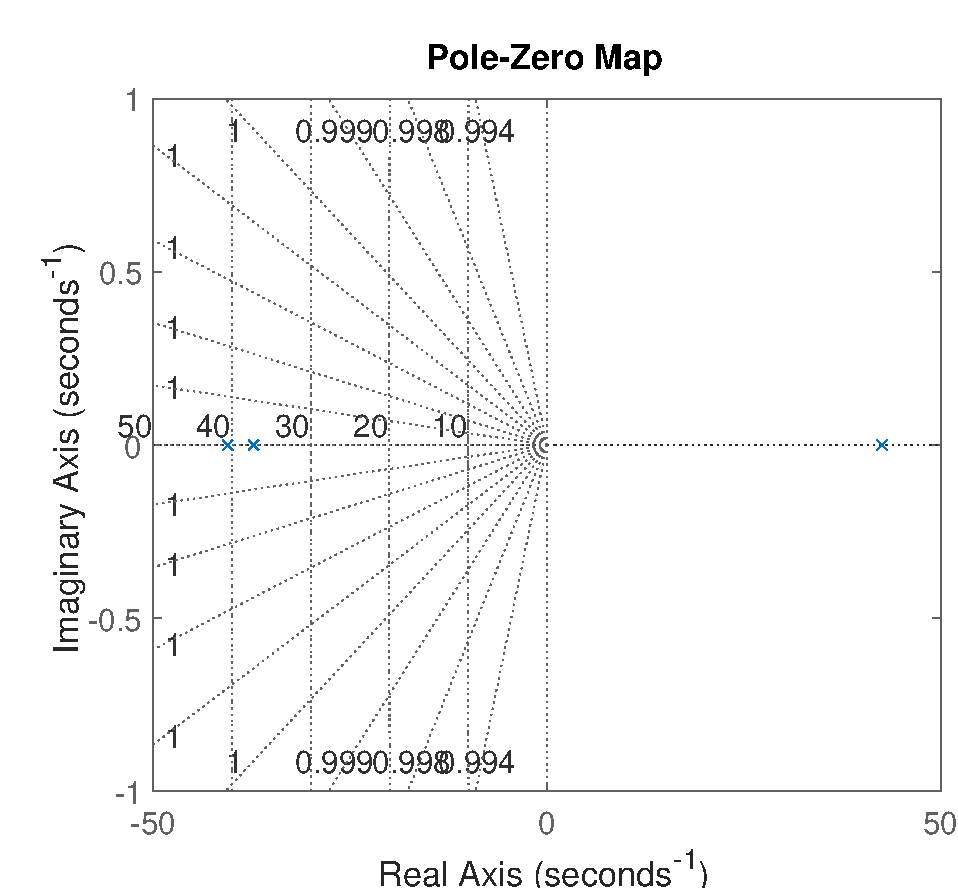
\includegraphics[width=0.5\textwidth]{./img/MATLAB/analysis/pole_zero_map.pdf}
    \caption{Pole-Zero Map}
    \label{fig:pole_zero_map}
\end{figure}

Notice that the system doesn't have any zeros, and as previously mentioned, one of the poles is located in the right-hand side of the complex plane, confirming the system's instability.


\paragraph{Root Locus}

Considering the unstable nature of the system, we perform a root locus analysis to identify potential gains that achieve a stable closed-loop system.
The root locus plot is shown in Figure \ref{fig:root_locus_plot}.

\begin{figure}[H]
    \centering
    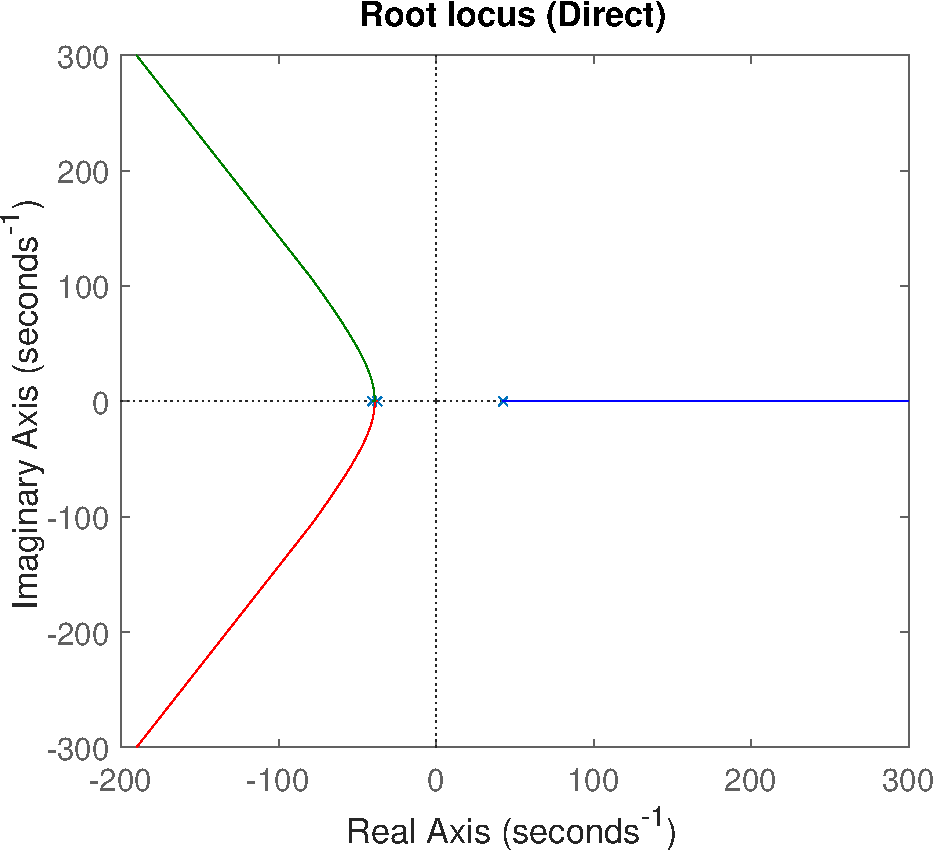
\includegraphics[width=0.47\textwidth]{./img/MATLAB/analysis/root_locus_direct.pdf}
    \hfill
    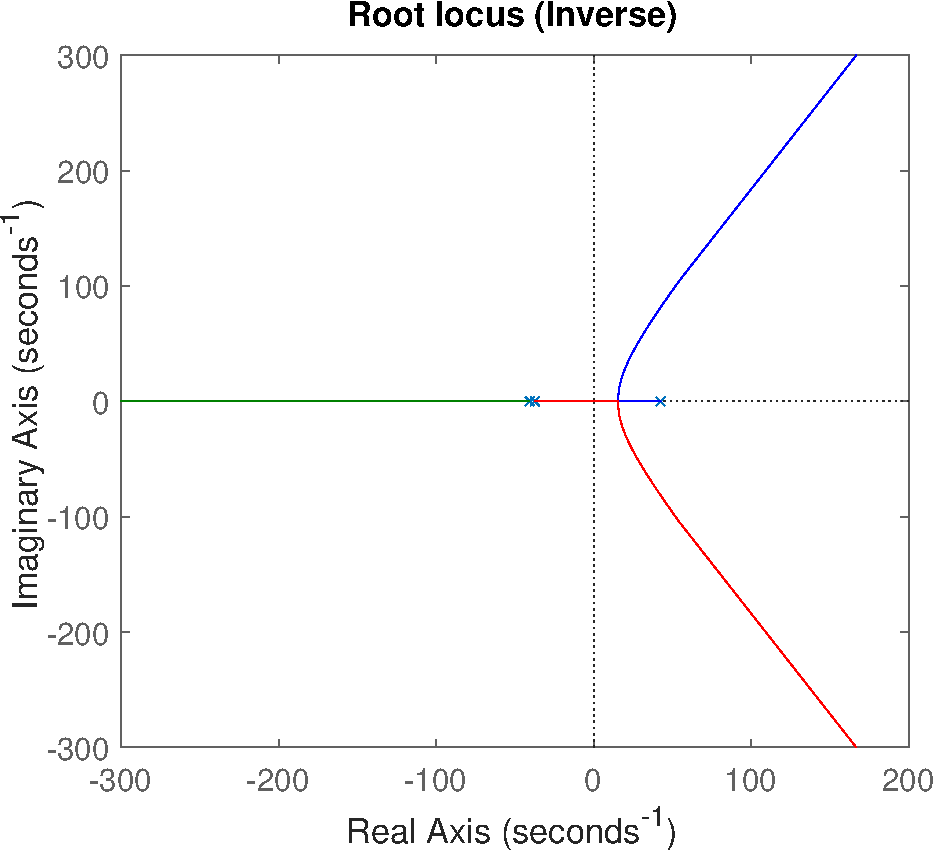
\includegraphics[width=0.47\textwidth]{./img/MATLAB/analysis/root_locus_inverse.pdf}
    \caption{Root Locus Plot}
    \label{fig:root_locus_plot}
\end{figure}

The root locus plot illustrates how the system poles migrate in the complex plane as the proportional gain of the controller is varied.

Again, we observe that one the three poles is unstable.
Moreover, we also notice that a simple proportional controller is not sufficient to stabilize the system, as the poles do not move to the left-hand side of the complex plane for any value of the gain $K$.



\paragraph{Bode Diagram}

To further analyze the stability of the system, we consider the Bode plot for the open-loop transfer function.
The Bode diagram is shown in Figure \ref{fig:bode_plot}.

\begin{figure}[H]
    \centering
    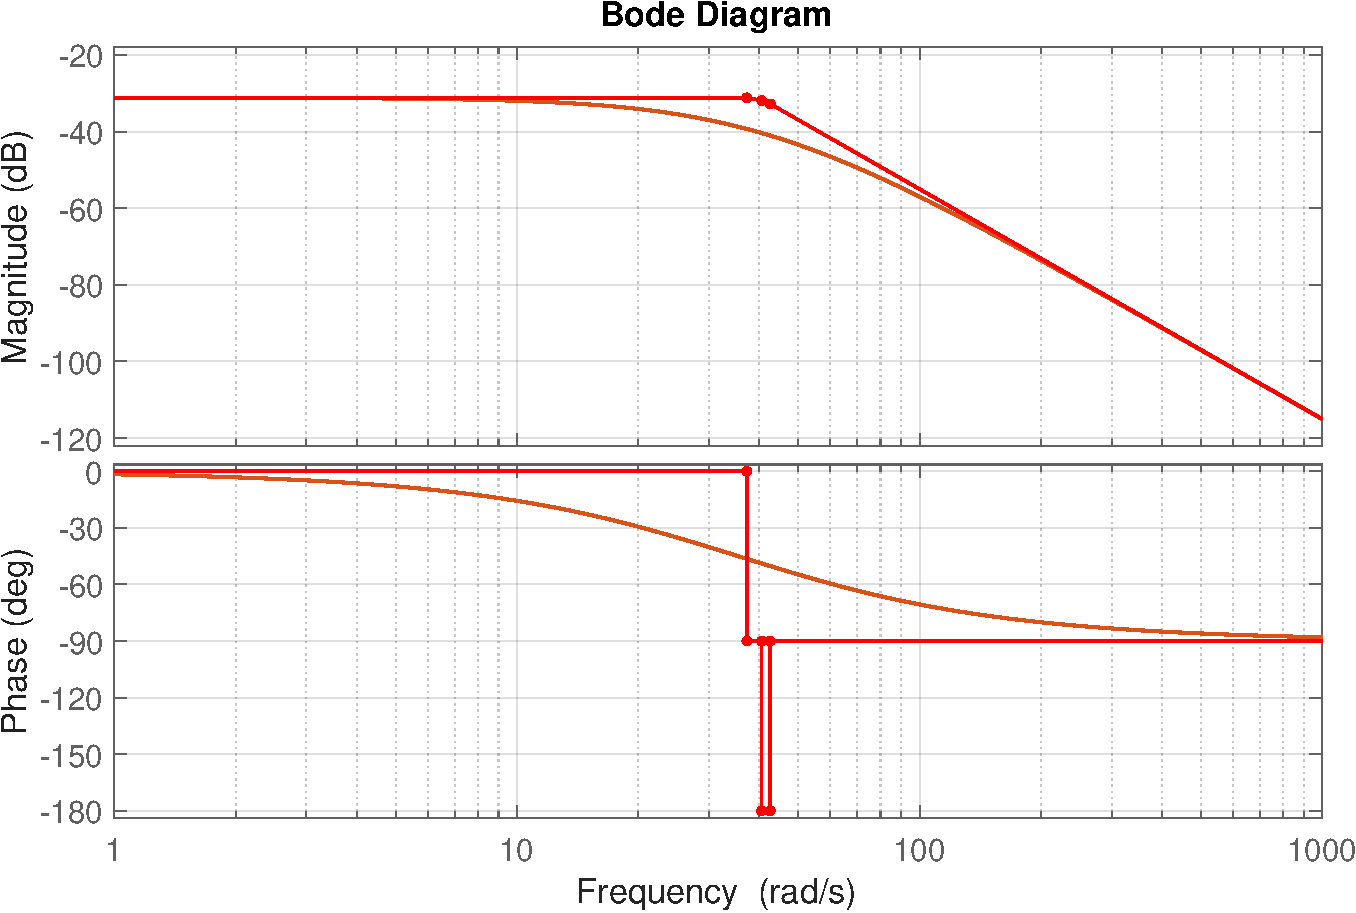
\includegraphics[width=0.8\textwidth]{./img/MATLAB/analysis/bode_plot.pdf}
    \caption{Bode Plot}
    \label{fig:bode_plot}
\end{figure}

Again, we observe that the system is unstable, as the gain margin is negative and the phase margin is less than $-180^{\circ}$.
\subsection{Levitation region}
\label{subsec:levitation_region}

From the analysis performed in Section \ref{subsec:force_analysis}, we can derive the levitation region of the system in which it's possible to maintain the ball in a levitated state provided that the force from the upper coil is greater than the gravitational force acting on the ball.

\begin{figure}[H]
    \centering
    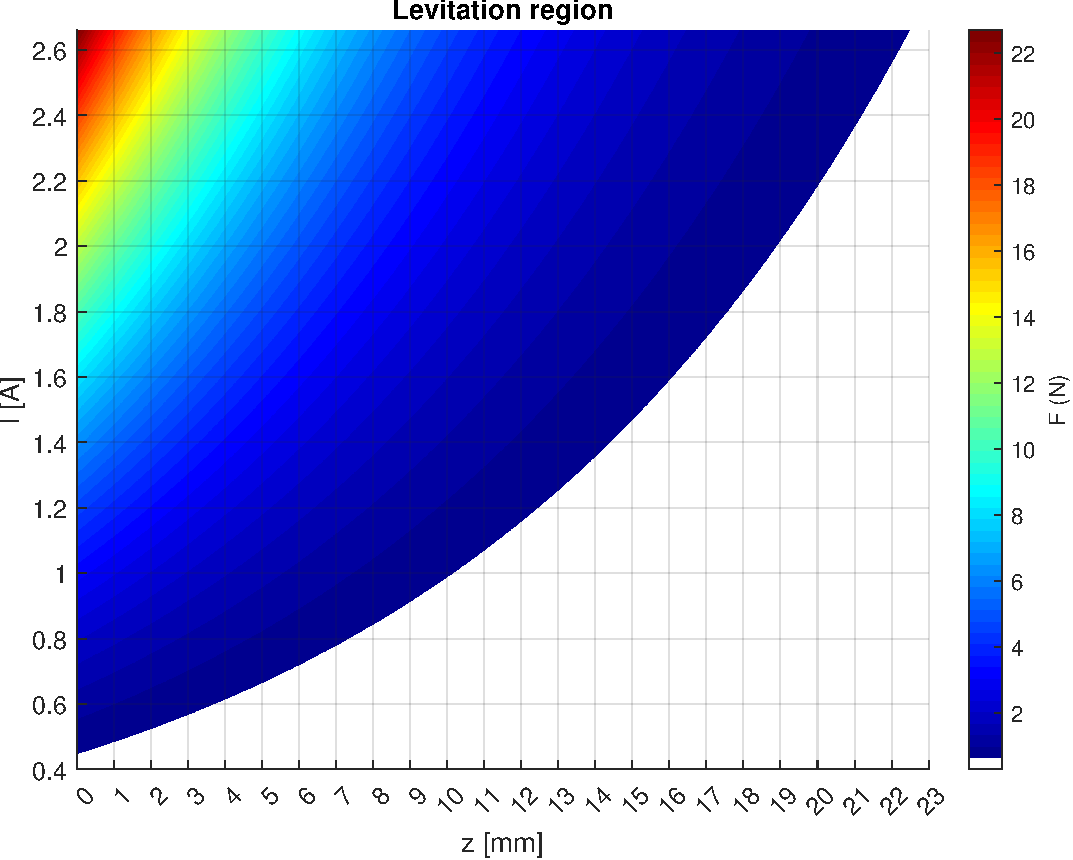
\includegraphics[width=0.7\textwidth]{./img/MATLAB/analysis/levitation_region.pdf}
    \caption{Levitation Region}
    \label{fig:levitation_region}
\end{figure}

From Figure \ref{fig:levitation_region}, it's also possible to see that the maximum distance from the upper coils before the ball falls is $z_{max} = 22.97 [mm]$ at values of the current equal to $I_{max} = 2.66 [A]$.